
\chapter[Bài tập: Mạch điện xoay chiều có\\ độ tự cảm của cuộn cảm biến thiên;\\Bài tập: Mạch điện xoay chiều có\\ điện dung của tụ điện biến thiên]{Bài tập: Mạch điện xoay chiều có độ tự cảm\\ của cuộn cảm biến thiên;\\Bài tập: Mạch điện xoay chiều có điện dung\\ của tụ điện biến thiên}
\section{Lý thuyết}
\subsection{Ứng dụng của hiện tượng cộng hưởng điện trong các bài toán về độ tự cảm của cuộn cảm biến thiên}
\subsubsection{Điều kiện xảy ra hiện tượng cộng hưởng điện khi $L$ thay đổi}
Để xảy ra hiện tượng cộng hưởng điện thì $Z_L = Z_C$, khi đó giá trị của độ tự cảm $L_\text{CH}$ ($L$ cộng hưởng) là
\begin{equation*}
	L_\text{CH}=\dfrac{1}{\omega ^2 C}.
\end{equation*}
\subsubsection{Có hai giá trị $L_1$, $L_2$ cho cùng một giá trị $I$, $\calP$. Tìm độ tự cảm $L_\text{CH}$ để trong mạch xảy ra hiện tượng cộng hưởng điện}
\begin{align*}
	I_1 &= I_2 \\
	\Leftrightarrow \dfrac{U}{\sqrt{R^2 + (Z_{L1}-Z_C)^2}}&=\dfrac{U}{\sqrt{R^2+(Z_{L2}-Z_C)^2}}\\
	\Rightarrow (Z_{L1}-Z_C)&=-(Z_{L2}-Z_C)\\
	\Leftrightarrow Z_C &= \dfrac{Z_{L1}+Z_{L2}}{2}.	
\end{align*}
Mà $Z_C = Z_{L\ \text{CH}}$ (cộng hưởng), nên suy ra
\begin{align*}
	Z_{L\ \text{CH}}&= \dfrac{Z_{L1}+Z_{L2}}{2} \\
	\Rightarrow {L_\text{CH}}&= \dfrac{L_1+L_2}{2}.
\end{align*}

\subsection{Ứng dụng phương pháp đại số trong các bài toán về độ tự cảm của cuộn cảm biến thiên}
\subsubsection{$Z_L$ biến thiên để điện áp hiệu dụng giữa 2 đầu cuộn cảm là lớn nhất ($U_{L\ \text{max}}$)}

\begin{center}
	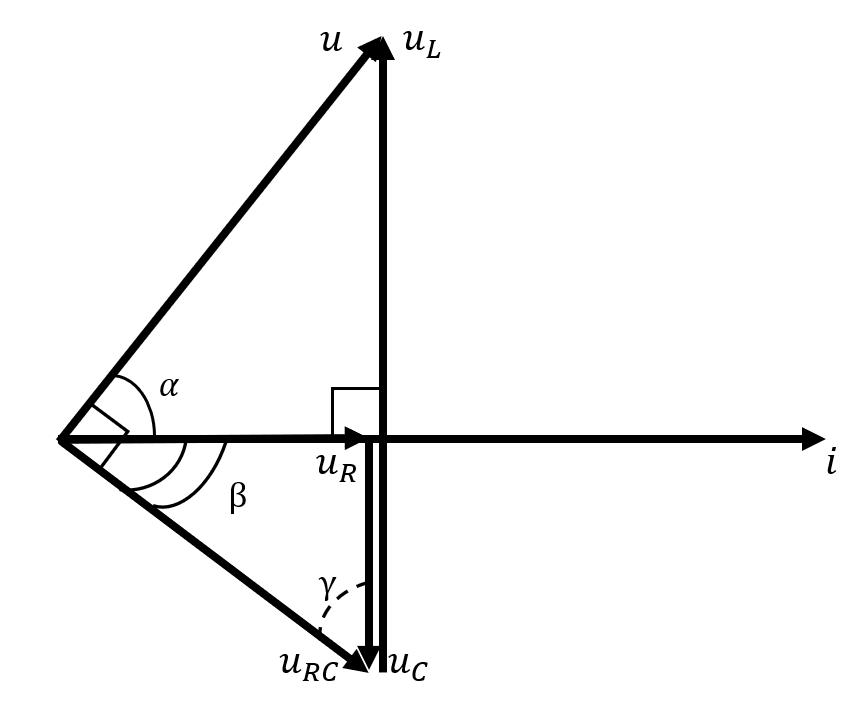
\includegraphics[scale=0.45]{../figs/VN12-PH-19-A-011-5-V2-1.png}
\end{center}

Áp dụng định lí hàm số sin trong tam giác, ta có:
\begin{equation*}
	\dfrac{U_L}{\sin(\alpha+\beta)}= \dfrac{U}{\sin \gamma}
	\Leftrightarrow U_L = \dfrac{U\sin(\alpha+\beta)}{ \sin \gamma}.
\end{equation*}

Giá trị $U_L$ lớn nhất khi $\sin(\alpha+\beta)=1$ hay $\alpha+\beta = \dfrac{\pi}{2}\ \text {rad}$, khi đó
\begin{equation*}
	U_{L\ \text{max}}=\dfrac{U}{\sin \gamma}.
\end{equation*}

Mà $\gamma = \dfrac{\pi}{2} - \beta$, nên $\sin \gamma = \cos \beta = \dfrac{U_R}{U_{RC}}$,
suy ra
\begin{equation*}
	U_{L\ \text{max}}=\dfrac{U}{\dfrac{U_R}{U_{RC}}}=U\dfrac{U_{RC}}{U_R}=U\dfrac{\sqrt{R^2 + Z_C^2}}{R}.
\end{equation*}

Mặt khác, ta có $U_{RC}^2 = U_L U_C$ (hệ thức lượng), nên
\begin{equation*}
	I^2 \left(\sqrt {R^2 + Z_C^2}\right)^2 = (I Z_L) (I Z_C)\Rightarrow Z_L=\dfrac{R^2 + Z_C^2}{Z_C}.
\end{equation*}

Vậy khi $Z_L=\dfrac{R^2 + Z_C^2}{Z_C}$ thì $U_{L\ \text{max}}=U\dfrac{\sqrt{R^2 + Z_C^2}}{R}$.
\luuy{Khi $U_{L\ \text{max}}$ thì $U_{RC}$ vuông pha với $u$.}
\subsubsection{Khi hai giá trị $L_1$ khác $L_2$ làm cho hai đầu cuộn dây có cùng $U_L$}

Hai giá trị cảm kháng làm điện áp hai đầu cuộn dây có cùng giá trị nên:
$$U_{L_1}=U_{L_2} \Rightarrow \dfrac{U}{\sqrt{R^2+(Z_{L_1}-Z_C)^2}}Z_{L_1}=\dfrac{U}{\sqrt{R^2+(Z_{L_2}-Z_C)^2}}Z_{L_2}$$
$$\Rightarrow [R^2+(Z_{L_2}-Z_C)^2]Z^2_{L_1} = [R^2+(Z_{L_1}-Z_C)^2]Z^2_{L_2}$$
$$\Rightarrow (R^2+Z_C^2)(Z^2_{L_1} - Z^2_{L_2})=2Z_{L_1}Z_{L_2} Z_C (Z_{L_1}- Z_{L_2}).$$

Do $Z_{L_1}$ khác $Z_{L_2}$, chia cả 2 vế cho $Z_{L_1}-Z_{L_2}$ ta có:
$$(R^2+Z_C^2)(Z_{L_1}+Z_{L_2})=2Z_{L_1}Z_{L_2} Z_C$$
$$\Rightarrow \dfrac{Z_{L_1}+Z_{L_2}}{Z_{L_1}Z_{L_2}} = 2 \dfrac{Z_C}{R^2+Z_C^2}$$
$$\Rightarrow \dfrac{1}{Z_{L_1}} + \dfrac{1}{Z_{L_2}}  = \dfrac{2}{Z_{L}} =2 \dfrac{Z_C}{R^2+Z_C^2}$$

Vậy $Z_L = \dfrac{2Z_{L_1}Z_{L_2}}{Z_{L_1}+Z_{L_2}} \Rightarrow L = \dfrac{2L_1L_2}{L_1+L_2}.$ với $L$ là giá trị cho $U_{L_\text{max}}$.
\subsection{Ứng dụng của hiện tượng cộng hưởng điện trong các bài toán về điện dung của tụ điện biến thiên}
\subsubsection{Điều kiện xảy ra hiện tượng cộng hưởng điện khi $C$ thay đổi}
Để xảy ra hiện tượng cộng hưởng điện thì $Z_L = Z_C$, khi đó giá trị của điện dung $C_\text{CH}$ ($C$ cộng hưởng) là
\begin{equation*}
	C_\text{CH}=\dfrac{1}{\omega ^2 L}.
\end{equation*}
\subsubsection{Có hai giá trị $C_1$, $C_2$ cho cùng một giá trị $I$, $\calP$. Tìm điện dung $C_\text{CH}$ để trong mạch xảy ra hiện tượng cộng hưởng điện}
\begin{align*}
	I_1 &= I_2 \\
	\Leftrightarrow \dfrac{U}{\sqrt{R^2 + (Z_{L}-Z_{C1})^2}}&=\dfrac{U}{\sqrt{R^2+(Z_{L}-Z_{C2})^2}}\\
	\Rightarrow (Z_{L}-Z_{C1})&=-(Z_{L}-Z_{C2})\\
	\Leftrightarrow Z_L &= \dfrac{Z_{C1}+Z_{C2}}{2}.	
\end{align*}
Mà $Z_L = Z_{C\ \text{CH}}$ (cộng hưởng), nên
\begin{align*}
	Z_{C\ \text{CH}}&= \dfrac{Z_{C1}+Z_{C2}}{2} \\
	\Rightarrow {C_\text{CH}}&= \dfrac{2C_1C_2}{C_1 + C_2}.
\end{align*}

\subsection{Ứng dụng phương pháp đại số trong các bài toán về điện dung của tụ điện biến thiên}
\subsubsection{Thay đổi $Z_C$ để điện áp hiệu dụng giữa 2 đầu tụ điện là lớn nhất ($U_{C\ \text{max}}$)}
\begin{center}
	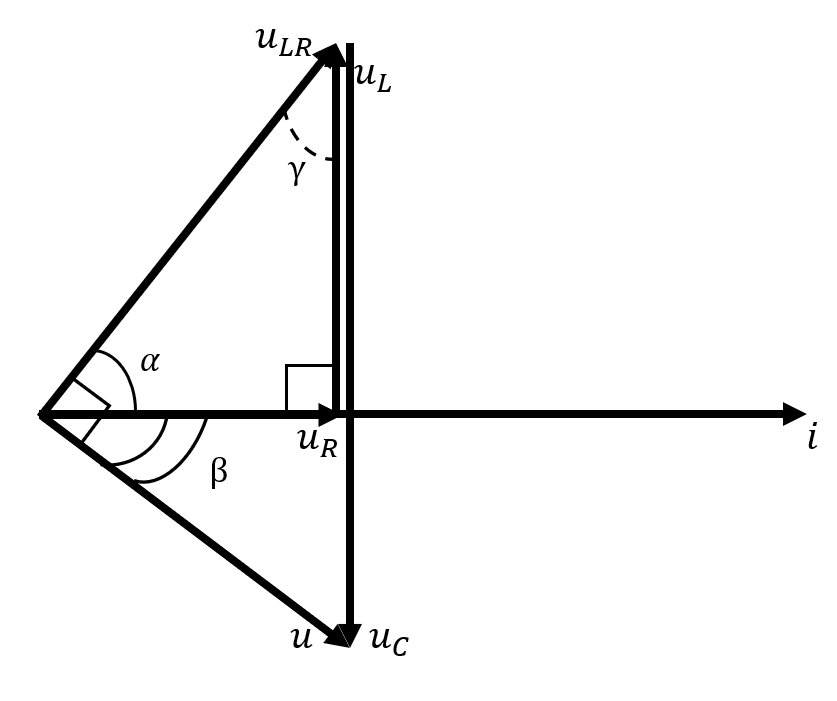
\includegraphics[scale=0.45]{../figs/VN12-PH-19-A-011-6-V2-1.png}
\end{center}
Áp dụng định lí hàm số sin trong tam giác, ta có:
\begin{equation*}
	\dfrac{U_C}{\sin(\alpha+\beta)}= \dfrac{U}{\sin \gamma}
	\Leftrightarrow U_C = \dfrac{U\sin(\alpha+\beta)}{ \sin \gamma}.
\end{equation*}

Giá trị $U_C$ lớn nhất khi $\sin(\alpha+\beta)=1$ hay $\alpha+\beta = \dfrac{\pi}{2}\ \text {rad}$, khi đó
\begin{equation*}
	U_{C\ \text{max}}=\dfrac{U}{\sin \gamma}.
\end{equation*}

Mà $\gamma = \dfrac{\pi}{2} - \alpha$, nên $\sin \gamma = \cos \alpha = \dfrac{U_R}{U_{LR}}$,
suy ra
\begin{equation*}
	U_{C\ \text{max}}=\dfrac{U}{\dfrac{U_R}{U_{LR}}}=U\dfrac{U_{LR}}{U_R}=U\dfrac{\sqrt{R^2 + Z_L^2}}{R}.
\end{equation*}

Mặt khác, ta có $U_{LR}^2 = U_L U_C$ (hệ thức lượng), nên
\begin{equation*}
	I^2 \left(\sqrt {R^2 + Z_L^2}\right)^2 = (I Z_L) (I Z_C)\Rightarrow Z_C=\dfrac{R^2 + Z_L^2}{Z_L}.
\end{equation*}

Vậy khi $Z_C=\dfrac{R^2 + Z_L^2}{Z_L}$ thì $U_{C\ \text{max}}=U\dfrac{\sqrt{R^2 + Z_L^2}}{R}$.
\luuy{Khi $U_{C\ \text{max}}$ thi $U_{RL}$ vuông pha với $u$}
\subsubsection{Khi hai giá trị $C_1$ khác $C_2$ làm cho hai đầu tụ điện có cùng $U_C$}

Hai giá trị dung kháng làm điện áp hai đầu tụ điện có cùng giá trị nên:
$$U_{C_1}=U_{C_2} \Rightarrow \dfrac{U}{\sqrt{R^2+(Z_{L}-Z_{C_1})^2}}Z_{C_1}=\dfrac{U}{\sqrt{R^2+(Z_{L}-Z_{C_2})^2}}Z_{C_2}$$
$$\Rightarrow [R^2+(Z_{L}-Z_{C_1})^2]Z^2_{C_1} = [R^2+(Z_{L}-Z_{C_2})^2]Z^2_{C_2}$$
$$\Rightarrow (R^2+Z_L^2)(Z^2_{C_1} - Z^2_{C_2})=2Z_{C_1}Z_{C_2} Z_L (Z_{C_1}- Z_{C_2}).$$

Do $Z_{C_1}$ khác $Z_{C_2}$, chia cả 2 vế cho $Z_{C_1}-Z_{C_2}$ ta có:
$$(R^2+Z_L^2)(Z_{C_1}+Z_{C_2})=2Z_{C_1}Z_{C_2} Z_L$$
$$\Rightarrow \dfrac{Z_{C_1}+Z_{C_2}}{Z_{C_1}Z_{C_2}} = 2 \dfrac{Z_L}{R^2+Z_L^2}$$
$$\Rightarrow \dfrac{1}{Z_{C_1}} + \dfrac{1}{Z_{C_2}}  = \dfrac{2}{Z_{C}} =2 \dfrac{Z_L}{R^2+Z_L^2}$$

Vậy $Z_C = \dfrac{2Z_{C_1}Z_{C_2}}{Z_{C_1}+Z_{C_2}} \Rightarrow C = \dfrac{C_1+C_2}{2}.$ với $C$ là giá trị cho $U_{C_\text{max}}$.

\section{Mục tiêu bài học - Ví dụ minh họa}
\begin{dang}{Ứng dụng của hiện tượng cộng hưởng điện trong các bài toán về độ tự cảm\\ của cuộn cảm biến thiên}
	\viduii{3}{ Một đoạn mạch AB mắc nối tiếp gồm: điện trở thuần $R$, tụ điện có điện dung $C$ và cuộn cảm thuần có độ tự cảm $L$ thay đổi được. Đặt vào hai đầu đoạn mạch AB điện áp xoay chiều $100\ \text{V} - 50\ \text{Hz}$. Điều chỉnh $L$ để $R^2 =\dfrac{\text{6,25}L}{C}$ và điện áp ở hai đầu cuộn cảm lệch pha so với điện áp ở hai đầu đoạn mạch AB góc $\dfrac{\pi}{2}$. Điện áp hiệu dụng ở hai đầu cuộn cảm là
		\begin{mcq}(4)
			\item 40 V.
			\item 30 V.
			\item 50 V.
			\item 20 V.
		\end{mcq}
		
	}
	{\begin{center}
			\textbf{Hướng dẫn giải}
		\end{center}
		Điện áp giữa hai đầu cuộn cảm lệch pha $\dfrac{\pi}{2}$ so với $i$.
		
		Điện áp giữa hai đầu cuộn cảm lệch pha 
		$\dfrac{\pi}{2}$ so với $u$.
		
		Suy ra: $i$ cùng pha $i$ nên xảy ra hiện tượng cộng hưởng.
		
		Vậy $U_R = U = 100\ \text{V}.$
		
		Theo đề bài ta có:
		$$R^2 =\dfrac{\text{6,25}L}{C} = \dfrac{\text{6,25}\omega L}{\omega C} = \text{6,25} Z_L Z_C =\text{6,25}Z_L^2 \Rightarrow Z_L =\text{0,4}R. $$
		
		Điện áp hiệu dụng ở hai đầu cuộn cảm là
		$$U_L =I Z_L = \dfrac{U}{R}Z_L = 40\ \text{V}.$$
		
		\textbf{Đáp án: A.}
	}
	\viduii{3}{ Đặt điện áp xoay chiều có giá trị hiệu dụng không đổi, tần số $\SI{50}{\hertz}$ vào hai đầu đoạn mạch mắc nối tiếp gồm điện trở thuần $R$, tụ điện có điện dung $C$ và cuộn cảm thuần có độ tự cảm thay đổi được. Điều chỉnh giá trị độ tự cảm $L$ thì thấy khi $L_1 = \SI{0.3}{\henry}$ hoặc $L_2 = \SI{0.5}{\henry}$ thì điện áp hiệu dụng giữa 2 đầu điện trở đều có giá trị bằng nhau. Tìm giá trị $L$ để cường độ dòng điện hiệu dụng trong mạch là lớn nhất.
		\begin{mcq}(4)
			\item $L=\SI{0.2}{\henry}$.
			\item $L=\SI{0.4}{\henry}$.
			\item $L=\SI{0.6}{\henry}$.
			\item $L=\SI{0.8}{\henry}$.
		\end{mcq}
		
	}
	{\begin{center}
			\textbf{Hướng dẫn giải}
		\end{center}
		Có hai giá trị của $L$ cho cùng một giá trị $U_R$, nên:
		\begin{align*}
			U_{R1}&=U_{R2} \\
			\Rightarrow I_1 &= I_2.
		\end{align*}
		
		Qua các bước chứng minh (như trên), ta được:
		\begin{equation*}
			L_\text{CH}=\dfrac{L_1+L_2}{2}=\SI{0.4}{\henry}.
		\end{equation*}
		
		\textbf{Đáp án: B.}
	}
\end{dang}
\begin{dang}{Ứng dụng phương pháp đại số\\ trong các bài toán về độ tự cảm\\ của cuộn cảm biến thiên}
	\viduii{3}{Cho mạch điện xoay chiều $R$, $L$, $C$ mắc nối tiếp có điện áp hai đầu đoạn mạch là $u=120\sqrt 2 \cos 100 \pi t \ \text {(V)}$. Biết $R=20\sqrt 3 \ \Omega$, $Z_C = 60\ \Omega$ và độ tự cảm $L$ thay đổi (cuộn dây thuần cảm). Xác định $L$ để $U_L$ cực đại và giá trị cực đại của $U_L$ bằng bao nhiêu?
		\begin{mcq}(2)
			\item $L=\dfrac{0,8}{\pi}\ \text H$, $U_{L\ \text {max}}=120\ \text V$.
			\item $L=\dfrac{0,6}{\pi}\ \text H$, $U_{L\ \text {max}}=240\ \text V$.
			\item $L=\dfrac{0,6}{\pi}\ \text H$, $U_{L\ \text {max}}=120\ \text V$.
			\item $L=\dfrac{0,8}{\pi}\ \text H$, $U_{L\ \text {max}}=240\ \text V$.
		\end{mcq}
		
	}
	{\begin{center}
			\textbf{Hướng dẫn giải}
		\end{center}
		Vẽ giản đồ vectơ trượt và qua các bước chứng minh (như trên), ta được:
		\begin{equation*}
			Z_L = \dfrac{R^2 + Z_C ^2}{Z_C} = 80\ \Omega \Rightarrow L = \dfrac{0,8}{\pi}\ \text H
		\end{equation*}
		và
		\begin{equation*}
			U_{L\ \text{max}}=U\dfrac{\sqrt{R^2 +Z_C ^2}}{R} = 240\ \text V.
		\end{equation*}
		
		\textbf{Đáp án: D.}
	}
	
	\viduii{3}{Cho mạch điện xoay chiều gồm RLC mắc nối tiếp,cuộn cảm thuần có độ tự cảm thay đổi được. Đặt vào hai đầu đoạn mạch điện áp xoay chiều $u = 100\sqrt 6 \cos100\pi t$. Điều chỉnh độ tự cảm để điện áp trên hai đầu cuộn cảm đạt giá trị cực đại là $U_{L_\text{max}}$ thì điện áp hiệu dụng trên hai đầu tụ điện là $U_C = 200\ \text{V}$. Giá trị $U_{L_\text{max}}$ là
		\begin{mcq}(4)
			\item 300 V.
			\item 100 V.
			\item 150 V.
			\item 250 V.
		\end{mcq}
	}
	{\begin{center}
			\textbf{Hướng dẫn giải}
		\end{center}
		
		Ta có $U_L =U_{L_\text{max}}$ khi
		$$ Z_L = \dfrac{R^2+Z_C^2}{Z_C} \Rightarrow U_LU_C = U_R^2 + U_C^2\ (1)$$
		
		Mặt khác: 
		$$U^2 =U^2_R +(U_L-U_C)^2 (2)$$
		
		Thay (1) vào (2) ta được:
		$$U^2_L -U_CU_L-U^2 =0\Leftrightarrow U^2_L -200U_L-30000 =0 (3)$$
		
		Giải (3) tìm được $U_L =300\ \text{V}$.
		
		\textbf{Đáp án: A.}
	}
	\viduii{3}{Cho mạch điện RLC mắc nối tiếp theo thứ tự $R, L, C$ trong đó cuộn dây thuần cảm có độ tự cảm $L$ thay đổi được. Đặt vào hai đầu đoạn mạch hiệu điện thế xoay chiều có tần số $f$. Thay đổi $L$ người ta thấy khi $L=L_1 = \dfrac{3}{\pi}\ \text{H}$	và khi $L=L_2 = \dfrac{1}{2\pi}\ \text{H}$  thì hiệu điện thế trên cuộn dây thuần cảm là như nhau. Để hiệu điện thế trên cuộn dây đạt cực đại thì $L$ có giá trị:
		\begin{mcq}(4)
			\item $\dfrac{7}{6\pi}\ \text{H}$.
			\item $\dfrac{6}{7\pi}\ \text{H}$.
			\item $\dfrac{6}{5\pi}\ \text{H}$.
			\item $\dfrac{5}{6\pi}\ \text{H}$.
		\end{mcq}
	}
	{\begin{center}
			\textbf{Hướng dẫn giải}
		\end{center}
		
		Để hiệu điện thế trên cuộn dây đạt cực đại thì $L$ có giá trị:
		
		$$Z_L = \dfrac{2Z_{L_1}Z_{L_2}}{Z_{L_1}+Z_{L_2}} \Rightarrow L = \dfrac{2L_1L_2}{L_1+L_2} = \dfrac{6}{7\pi}\ \text{H}.$$  
		
		\textbf{Đáp án: B.}
	}
\end{dang}
\begin{dang}{Ứng dụng của hiện tượng cộng hưởng điện trong các bài toán về điện dung\\ của tụ điện biến thiên}
	\viduii{2}{Trong mạch điện xoay chiều biến thiên với tần số góc $\omega$ chứa $R$, $L$, $C$ mắc nối tiếp. Cho $R$, $L$, $\omega$ không đổi. Thay đổi $C$ đến khi $C=C_0$ thì cường độ dòng điện trong mạch đạt giá trị cực đại. Khi đó
		\begin{mcq}(2)
			\item $C_0 = \dfrac{1}{\omega ^2 L}$.
			\item $C_0 = \dfrac{R^2 + Z_C ^2}{\omega L}$.
			\item $C_0= \dfrac{1}{(\omega L)^2} \dfrac{R^2 +Z_C ^2}{\omega L}$.
			\item $C_0= \dfrac{1}{(\omega L)^2}$.
		\end{mcq}
	}
	{\begin{center}
			\textbf{Hướng dẫn giải}
		\end{center}
		
		Thay đổi $C$ đến khi cường độ dòng điện trong mạch đạt giá trị cực đại thì xảy ra hiện tượng cộng hưởng, khi đó $C_0 = \dfrac{1}{\omega ^2 L}$.
		
		\textbf{Đáp án: A.}
	}
	
	\viduii{3}{Mạch $RLC$ nối tiếp, $C$ thay đổi được. Khi $C_1=\dfrac{2\cdot 10^{-4}}{\pi}\ \text{F}$ hoặc $C_2= \dfrac{10^{-4}}{\text{1,5}\pi}\ \text{F}$ thì có cùng công suất của mạch có giá trị như nhau. Hỏi với giá trị nào của $C$ thì công suất trong mạch cực đại?
		\begin{mcq}(2)
			\item $C = \dfrac{ 10^{-4}}{2\pi}\ \text{F}$.
			\item $C = \dfrac{ 10^{-4}}{\pi}\ \text{F}$.
			\item $C = \dfrac{ 2\cdot 10^{-4}}{3\pi}\ \text{F}$.
			\item $C = \dfrac{\cdot 3 \cdot 10^{-4}}{2\pi}\ \text{F}$.
		\end{mcq}
		
	}
	{\begin{center}
			\textbf{Hướng dẫn giải}
		\end{center}
		
		Để công suất trong mạch đạt cực đại thì $C$
		
		\begin{align*}
			Z_{C\ \text{CH}}&= \dfrac{Z_{C1}+Z_{C2}}{2} \\
			\Rightarrow {C_\text{CH}}&= \dfrac{2C_1C_2}{C_1 + C_2} = \dfrac{10^{-4}}{\pi}\ \text{F}.
		\end{align*}
		
		\textbf{Đáp án: B.}
	}
	
	
\end{dang}


\begin{dang}{Ứng dụng phương pháp đại số\\ trong các bài toán về điện dung\\ của tụ điện biến thiên}
	\viduii{3}{Cho mạch điện xoay chiều $RLC$ có: $R = 100\ \Omega; L = \dfrac{2}{\pi}\ \text{H}$, điện dung $C$ của tụ điện biến thiên. Đặt vào hai đầu mạch điện áp $u = 200\sqrt 2 \cos 100\pi t \text{V}$. Tính $C$ để điện áp giữa hai đầu tụ điện đạt giá trị cực đại.
		\begin{mcq}(2)
			\item $C = \dfrac{ 10^{-4}}{2\pi}\ \text{F}$.
			\item $C = \dfrac{ 10^{-4}}{\text{2,5}\pi}\ \text{F}$.
			\item $C = \dfrac{ 10^{-4}}{4\pi}\ \text{F}$.
			\item $C = \dfrac{\cdot 10^{-2}}{2\pi}\ \text{F}$.
		\end{mcq}
	}
	{\begin{center}
			\textbf{Hướng dẫn giải}
		\end{center}
		
		Cảm kháng của cuộn dây:
		$$ Z_L = L \omega = 200\ \Omega$$
		
		Dung kháng của tụ điện để điện áp giữa hai đầu tụ điện đạt giá trị cực đại
		
		$$Z_C=\dfrac{R^2 + Z_L^2}{Z_L} = 250\ \Omega.$$
		
		Vậy điện dung của tụ:
		$$C =\dfrac{1}{Z_C \omega} = \dfrac{10^{-4}}{\text{2,5}\pi}\ \text{H}.$$
		
		\textbf{Đáp án: B.}
	}
	
	\viduii{3}{Đặt điện áp xoay chiều vào hai đầu đoạn mạch $R, L, C$ nối tiếp có C thay đổi thì thấy khi $C_1 = \dfrac{10^{-4}}{\pi}\ \text{F}$ và $C_2 = \dfrac{10^{-4}}{2\pi}\ \text{F}$ thì điện áp hiệu dụng đặt vào tụ $C$ không đổi. Để điện áp hiệu dụng đó đạt cực đại thì giá trị $C$ là
		\begin{mcq}(2)
			\item $C = \dfrac{3 \cdot 10^{-4}}{4\pi}\ \text{F}$.
			\item $C = \dfrac{ 10^{-4}}{3\pi}\ \text{F}$.
			\item $C = \dfrac{3 \cdot 10^{-4}}{2\pi}\ \text{F}$.
			\item $C = \dfrac{ 2\cdot 10^{-4}}{3\pi}\ \text{F}$.
		\end{mcq}
	}
	{\begin{center}
			\textbf{Hướng dẫn giải}
		\end{center}
		
		Để điện áp hiệu dụng đó đạt cực đại thì giá trị $C$ là:
		
		$$C = \dfrac{C_1+C_2}{2}= \dfrac{3 \cdot 10^{-4}}{4\pi}\ \text{F}.$$
		
		\textbf{Đáp án: A.}
	}
\end{dang}